% \iffalse meta-comment
% 
% Copyright (C) 2007, 2008 by Xu Yuan <xuyuan.cn@gmail.com>
%                             SONG Yiha <syhannnn@gmail.com>
% $Id$
% 
% This file is part of the seuthesis package project.
% http://seuthesis.googlecode.com/
% ---------------------------------------------------
% This file may be distributed and/or modified under the
% conditions of the GNU General Public License v3
% of this license or (at your option) any later version.
% The latest version of this license is in:
% 
% http://www.gnu.org/licenses/gpl.html
% 
% \fi
%
% \CheckSum{0}
% \CharacterTable
%  {Upper-case    \A\B\C\D\E\F\G\H\I\J\K\L\M\N\O\P\Q\R\S\T\U\V\W\X\Y\Z
%   Lower-case    \a\b\c\d\e\f\g\h\i\j\k\l\m\n\o\p\q\r\s\t\u\v\w\x\y\z
%   Digits        \0\1\2\3\4\5\6\7\8\9
%   Exclamation   \!     Double quote  \"     Hash (number) \#
%   Dollar        \$     Percent       \%     Ampersand     \&
%   Acute accent  \'     Left paren    \(     Right paren   \)
%   Asterisk      \*     Plus          \+     Comma         \,
%   Minus         \-     Point         \.     Solidus       \/
%   Colon         \:     Semicolon     \;     Less than     \<
%   Equals        \=     Greater than  \>     Question mark \?
%   Commercial at \@     Left bracket  \[     Backslash     \\
%   Right bracket \]     Circumflex    \^     Underscore    \_
%   Grave accent  \`     Left brace    \{     Vertical bar  \|
%   Right brace   \}     Tilde         \~}
%
%
% \iffalse
%<*driver> 
\documentclass{seuthesis}
\usepackage{color}
\usepackage{manfnt}
\usepackage{verbatim}

% 在本文档中使用的宏
\newcommand{\bs}{\symbol{'134}}%Print backslash
\renewenvironment{quote}
{
  \color{magenta}
  {\small\textlhdbend}
  \kai
}{}
\newcommand{\IndexOpt}[1]{\index{\texttt{#1}}\texttt{#1}}
\newcommand{\IndexCmd}[1]{\index{\texttt{\bs #1}}}
\newcommand{\CmdMacro}[2]{\fbox{\texttt{\IndexCmd{#1}\bs #1#2}}}
\newcommand{\IndexEnv}[1]{\index{\texttt{\bs begin\{#1\}}}}
\newcommand{\EnvMacro}[2]{\fbox{\texttt{\IndexEnv{#1}\bs begin\{#1\}#2}}}

\begin{document}
\GetFileInfo{seuthesis.cls}

\categorynumber{000} % 分类采用《中国图书资料分类法》
\UDC{000} %《国际十进分类法UDC》的类号
\secretlevel{公开} %学位论文密级分为“公开”、“内部”、“秘密”和“机密”四种
\studentid{050962} %学号要完整,前面的零不能省略。

\title{\seuthesis{}~宏包(\fileversion版)} % 中文标题
{——东南大学学位论文~\LaTeX{}~模板} % 中文副标题
{The \seuthesis{} class (version \fileversion)} % 英文标题
{--- The \LaTeX{} template for thesis of Southeast University}%英文副标题

\author{许~元}{XU Yuan}

\advisor{导师姓名}{教授}{Advisor's Name}{Prof.}
\coadvisor{副导师}{副教授}{Co-advisor's Name}{Associate Prof.}
\major{\LaTeX}
\submitdate{2007年12月20日}{December 20, 2007}
\defenddate{2050年7月7日}
\authorizedate{2050年7月7日}
\department{自动化学院}{School of Automation}
\date{\today}

\maketitle

\begin{abstract}{\LaTeX{}~模板,东南大学学位论文}

  \TeX{} 是一个排版系统,可以把文章做成书那种效果。因此~\TeX{}非常适合
  用来写学术论文和书籍。\seuthesis{}是按照东南大学研究生院和教务处对学
  位论文的要求设计和实现的\LaTeX{}模板,帮助东南大学学生以专业排版水平
  来完成学位论文。

  本文既是\seuthesis{}使用手册也是范例,建议在使用\seuthesis{}之前阅
  读。
\end{abstract}

\begin{englishabstract}{\LaTeX{} template, thesis of Southeast
    Universiy} 

  \TeX is a typesetting system, it can make article as good as
  published book. Therefore, \TeX is very suitable for writing
  academic papers and books. \seuthesis{} is designed and implemented
  as a \LaTeX template to help studnets writing degree thesis in a
  professional typesetting, according to the requirements of Southeast
  University.

  This paper is \seuthesis{} user manual and also the sample
  document, it is better to be read before using \seuthesis{}.
\end{englishabstract}

\begin{terminology}
  \begin{table}
    \centering
    \caption{本论文专用术语(符号、变量、缩略词等)的注释表}
    \label{tab:terminology}
    \begin{tabular}{l|l}
      \noalign{\hrule height 1.2pt}
      符号、变量、缩略词等 & 涵义 \\
      \hline
      \textcolor{magenta}{{\small\textlhdbend}\kai 洋红色楷体字} & 引用《东南大学研究生学位论文格式规
      定》\cite{seugs:standard}原文\\
      \CmdMacro{命令}{\{参数\}} & 本宏包所支持的命令和参数\\
      \noalign{\hrule height 1.2pt}
    \end{tabular}
  \end{table}
\end{terminology}

\begin{Main}

  \chapter{简介} 
  \label{cha:intro}

  在硕士论文完成之际,\seuthesis{}的第一个完整版也诞生了,同时支
  持~UNICODE~和~GBK~编码,宋翊涵同学为模板加入了对东南大学本科论文的支
  持。模板的格式尽量满足研东南大学究生院和教务处的要求,当然由于水平有
  限其中错漏在所难免,我们已在google建立项
  目:\url{http://seuthesis.googlecode.com/},欢迎东大的\LaTeX{}er一起参
  加开发和完善。

  如果您对开发和完善\seuthesis{}感兴趣、有任何想法或建议,请与我
  们联系。

  \section{版权声明}
  \begin{flushleft}
    \begin{tabular*}{1.0\linewidth}{lcl}
      版权所有\textcopyright 2007, 2008 & 许元 & \url{(xuyuan.cn@gmail.com)} \\
      & 宋翊涵 & \url{(syhannnn@gmail.com)} \\
    \end{tabular*}
  \end{flushleft}

  这一程序是自由软件,你可以遵照自由软件基金会发布的《 GNU通用公共许可
  证条款第三版》来修改和重新发布这一程序,或者(根据您的选择)用任何更新
  的版本。发布这一程序的目的是希望它有用,但没有任何担保。甚至没有适合
  特定目的的隐含的担保。更详细的情况请参阅《GNU通用公共许可
  证》\footnote{\url{http://www.gnu.org/licenses/gpl.html}}。

  \section{版本历史}
  \begin{description}
  \item[1.1] 2008/05/16,增加对东南大学本科论文的支持。
  \item[1.0] 2008/03/19,第一个完整版,包含了参考文献格式等完善。
  \item[0.2] 2007/12/23,增加unicode支持。
  \item[0.1] 2007/12/22,增加文档和示例。
  \item[0.0] 2007/12/02,初始版本。
  \end{description}

  \chapter{下载和安装}
  \label{cha:download-install}
  \section{发布版本}
  各个发布的版本可以到本项目在Google的project中找到,或者直接访问
  \url{http://code.google.com/p/seuthesis/downloads/list}下载。
  \section{开发版本}
  最新的正在开发中的版本可以通过~svn~下载,使用如下命令:
  \begin{flushleft}
    \texttt{svn checkout http://seuthesis.googlecode.com/svn/trunk/
      seuthesis-read-only}
  \end{flushleft} 详细信息请参考~Google~给出的~svn~访问方
  法\footnote{\url{http://code.google.com/p/seuthesis/source}}。

  \section{安装}
  \label{sec:install}
  将宏包中的文件与~\TeX{}~主文件放在同一目录下即可,当然也可以安装
  到~\TeX{}~系统中。

  本模板在~{\sc Suse 10.2}~系统下
  的~\texttt{tetex}~和~\texttt{texlive2007}~下编译通过。如有您在使用中有
  任何问题,欢迎与我联系。

  \chapter{使用说明}
  \begin{quote}
    学位论文应包括:
    \begin{enumerate}
    \item 中文封面;
    \item 英文页面;
    \item 论文独创性声明和使用授权声明;
    \item 中文内容提要及关键词;
    \item 英文内容提要及关键词;
    \item 目录;
    \item 正文;
    \item 致谢;
    \item 参考文献
    \end{enumerate}
    等7大要素并按此顺序排列。其他可以选择添加的内容有:
    \begin{itemize}
    \item 位于目录之后的内容:符号、变量、缩略词等本论文专用术语的注释表;
    \item 参考文献后按序排列的内容:
      \begin{enumerate}
      \item 附录;
      \item 索引(中、英文);
      \item 作者简介(包括在学期间发表的论文和取得的学术成果清单);
      \item 后记。
      \end{enumerate}
    \end{itemize}
  \end{quote}

  首先要在你的~\TeX{}~文件中使用本宏
  包:\CmdMacro{documentclass}{[\textit{选项}]\{seuthesis\}} 其中
  \texttt{选项}请参考\refsec{sec:use:opt}。然后在导言区中加入自己需要的
  宏包等,接着使用\CmdMacro{begin\{document\}}{}开始写论文,主要还要在
  最有用\CmdMacro{end\{document\}}{}结尾。

  在论文的一开始需要通过宏包的命令设置论文的题目、作者等,具体命令和参
  数参考\refsec{sec:use:cover}、\refsec{sec:use:abstract}。这些都设置好
  了之后使用\CmdMacro{maketitle}{}来生成封面、目录等,所以这条命令在设
  置之后正文开始之前使用,后面就可以开始论文了。

  \section{例子} 也许一个例子更能说清楚,下面就是使用本宏包的简要例子。
  这个例子就是宏包中的~\texttt{sample.tex}~文件,可以使用~\texttt{make
    sample}~命令来编译这个例子。

  \verbatiminput{sample}

  \section{选项}
  \label{sec:use:opt}
  \subsection{编码选项}
  \newcommand{\OPTunicode}{\IndexOpt{unicode}}
  \newcommand{\OPTgbk}{\IndexOpt{gbk}}
  \begin{description}
  \item[\OPTunicode] (默认)使用~UNICODE~编码;
  \item[\OPTgbk] 使用~GBK~编码。 
  \end{description}
  \subsection{学位选项}
  \newcommand{\OPTbachelor}{\IndexOpt{bachelor}}
  \newcommand{\OPTmaster}{\IndexOpt{master}}
  \newcommand{\OPTdoctor}{\IndexOpt{doctor}}
  \begin{description}
  \item[\OPTbachelor] 学士学位;
  \item[\OPTmaster] 硕士学位(默认);
  \item[\OPTdoctor] 博士学位。
  \end{description}

  \section{封面}
  \label{sec:use:cover} 使用\CmdMacro{maketitle}{}来生成中、英文封面以及
  《论文独创性声明和使用授权声明》,但是在调用\CmdMacro{maketitle}{}之前进
  行相关设置,包括姓名、论文题目等。下面详细说明相关设置命令。由于本科
  论文的封面和研究生论文的封面有很大差异,所以有些命令只在研究生论文中
  起作用,而有些只在本科论文中才需要。

  \subsection{分类号}
  \CmdMacro{categorynumber}{\{分类号\}},分类采用《中国图书资料分类法》。
  \subsection{UDC类号}
  \CmdMacro{UDC}{\{《国际十进分类法UDC》的类号\}}
  \subsection{论文保密等级}
  \CmdMacro{secretlevel}{\{学位论文密级\}},分为“公开”、“内部”、“秘密”和“机
  密”四种。
  \subsection{学号}
  \CmdMacro{studentid}{\{学号\}},研究生院要求学号要完整,前面的零不能省略。

  \subsection{论文标题} 
  \CmdMacro{title}{\{论文中文标题\}\{中文副标题\}\{论文英文标题\}\{英文副标题\}}

  \begin{quote}
    论文的主标题(第一行)。论文题目是论文全貌的集中体现,应能概括整个论文
    最重要的内容,命题必须确切、简明,题目应力求简单,也不应宽泛笼统,应能
    看出论文的实质性内容和工作重心。中文题名一般不超过20个汉字,必要时可加
    副题名。副题名可另起一行,用破折号与主题名隔开。题名中应避免使用非公知
    公用的缩略语、字符、代号以及结构式和公式。
  \end{quote}

  \subsection{作者}
  \CmdMacro{author}{\{作者中文姓名\}\{作者英文姓名\}}。

  \begin{quote}
    中国姓名译为英文时用汉语拼音,按照姓前名后的原则,姓、名均用全名,不宜
    用缩写。姓全用大写,名的第一个字母大写,名用双中文字时两个字的拼音之间
    可以不用短划线,但容易引起歧义时必须用短划线。例如“冯长根”译为“FENG
    Changgen”或“FENG Chang-gen”,而“冯长安”则必须译为“FENG
    Chang-an”。
  \end{quote}

  \subsection{导师}
  \CmdMacro{advisor}{\{导师中文姓名\}\{导师职称(教授、副教授等)\}\{导师英
    文姓名\}\{导师职称英文\}}

  另外如果有副导师,使用

  \CmdMacro{coadvisor}{\{副导师中文姓名\}\{副导师职称(教授、副教授等)\}\{副导师英
    文姓名\}\{副导师职称英文\}}

  \subsection{院系和专业}
  \CmdMacro{department}{\{院系中文名\}\{院系英文名\}}

  \CmdMacro{major}{[宽度]\{专业名称(中文)\}},其中宽度选项只在本科论
  文中有效。

  \subsection{日期}
  \subsubsection{论文提交日期}
  \CmdMacro{submitdate}{\{论文提交日期中文\}\{论文提交日期英文\}}
  \subsubsection{论文答辩日期}
  \CmdMacro{defenddate}{\{论文答辩日期中文\}}
  \subsubsection{学位授予日期}
  \CmdMacro{authorizedate}{\{学位授予日期中文\}}
  \subsubsection{论文完成日期}
  \CmdMacro{date}{\{论文完成日期中文\}}
  \subsubsection{起讫日期}
  \CmdMacro{duration}{\{论文开始时间——论文完成时间\}},本科论文需要。
  \subsection{答辩委员会主席}
  \CmdMacro{committeechair}{\{答辩委员会主席姓名、职称\}}
  \subsection{评阅人}
  \CmdMacro{reader}{\{评阅人甲姓名、职称\}\{评阅人乙姓名、职称\}}
  \subsection{学位授予单位}
  \CmdMacro{authorizeorganization}{\{学位授予单位\}},默认为“东南大学”。
  \subsection{设计地点}
  \CmdMacro{address}{\{设计地点\}},本科论文需要。

  \section{摘要和关键词}
  \label{sec:use:abstract}
  摘要的内容需要放置在环境中,而关键字是作为环境的参数设置的:

  \EnvMacro{abstract}{\{中文关键字\}}

  \EnvMacro{englishabstract}{\{英文关键字\}}

  \begin{quote}
    论文摘要包括题名、硕士(博士)研究生姓名、导师姓名、学校名称、正文、
    关键词。中文约500字左右,英文约200~300词左右,二者应基本对应。它是论
    文内容的高度概括,应说明研究目的、研究方法、成果和结论,要突出本论文
    的创造性成果或新的见解、用语简洁、准确,并在论文摘要后注明本文的关键
    词3至8个。关键词应为公知公用的词和学术术语,不可采用自造字词和略写、
    符号等,词组不宜过长。
  \end{quote}


  \begin{quote}
    英文摘要采用第三人称单数语气介绍该学位论文内容,目的是便于其他文摘摘录,
    因此在写作英文文摘时不宜用第一人称的语气陈述。叙述的基本时态为一般现在
    时,确实需要强调过去的事情或者已经完成的行为才使用过去时、完成时等其他
    时态。可以多采用被动语态,但要避免出现用“This paper”作为主语代替作者
    完成某些研究行为。
  \end{quote}

  \section{本论文专用术语的注释表} 
  术语注释表为可选内容,需要放置在环境变量中:
  \EnvMacro{terminology}{[标题]}
  其中,\emph{标题}默认值为“本论文专用术语的注释表”。

  \begin{quote}
    如果有必要可以设置本论文专用术语(符号、变量、缩略词等)的注释表。此部
    分内容可根据论文中采用的符号、变量、缩略词等专用术语加以定义和注释,以
    便于论文阅读和迅速查出某符号的明确含义。
  \end{quote}

  \section{正文}
  正文需要放置在\EnvMacro{Main}{}环境中。


  \begin{quote}
    正文是学位论文的主体。内容可因研究课题的性质不同而有所变化。一般可包括:
    文献综述、理论基础、计算方法、实验方法、经过整理加工的实验结果的分析讨
    论、见解和结论。
  \end{quote}

  \begin{quote}
    正文一律用阿拉伯数字编排页码,页码在底部居中。正文之前的摘要、目录等内
    容单独编排罗马数字页码。
  \end{quote}

  \subsection{绪论(前言)}

  \begin{quote}
    本研究课题国内外已有的重要文献的扼要概括,阐明研究此课题的目的、意义,
    研究的主要内容和所要解决的问题。本研究工作在国民经济建设和社会发展中的
    理论意义与实用价值。
  \end{quote}

  \subsection{文献综述}

  \begin{quote}
    在查阅国内外文献和了解国内外有关科技情况的基础上,围绕课题涉及的问题,
    综述前人工作情况,达到承前启后的目的。要求:
    \begin{itemize}
    \item 总结课题方向至少10年以来的国内外动态;
    \item 明确前人的工作水平;
    \item 介绍目前尚存在的问题;
    \item 说明本课题的主攻方向。
    \end{itemize}
    文献总结应达到可独立成为一篇综述文章的要求。
  \end{quote}

  \subsection{理论分析、数值计算或统计分析}

  \begin{quote}
    利用研究生本人所掌握的理论知识对所选课题进行科学地、严密地理论分析、数
    值计算或统计分析,剖析课题,提出自己的见解。
  \end{quote}

  \subsection{实验原理、实验方法及实验装置}

  \begin{quote}
    学位论文要求对实验原理、方法、装置、步骤和有关参数有较详细的阐述,以便
    评阅人及答辩委员会审核实验的可靠性,并能对试验进行重复以便验证结果的可
    靠性,也为以后的研究者提供一个较完整的研究方法。
  \end{quote}

  \subsection{实验结果及讨论分析}

  \begin{quote}
    列出数据的图或表,并对数据结果进行讨论,对比分析、结果推论要严格准确,
    避免采用模棱两可的评定语言。对反常的数据要保留并做解释或者说明,不可随
    意剔除数据做出有违科学公正的行为。
  \end{quote}


  \subsubsection{引用}

  研究生院规定引用参考文献采用的上标格式,应使用\CmdMacro{cite}{\{文献标
    题\}}命令,其效果是~\cite{seugs:standard}~。

  但是有时候又需要普通引用,这时使用\CmdMacro{citet}{\{文献标题\}}命
  令,其效果是~\citet{seugs:standard}~。

  引用文中的图和表使用\CmdMacro{autoref}{\{lable\}}命令,其效果
  是\autoref{tab:terminology}。

  引用文中某一章使用\CmdMacro{refchapter}{\{lable\}}命令,其效果
  是\refchapter{cha:intro}。

  引用文中某一节使用\CmdMacro{refsec}{\{lable\}}命令,其效果
  是\refsec{sec:install}。

  \begin{quote}
    引用的别人的研究成果及数据应加注参考文献,较长的公式推导可列入附录。采
    纳文献及引用数据应为可以公开并能重复查到的文献资源,并提供准确出处(如
    页码或图表序号等)。正文引用文献一律用右上角方括号内的次序号(阿拉伯数
    字)(用“上标”格式)。
  \end{quote}

  \section{致谢} 

  在正文结束之后(即\CmdMacro{end\{Main\}}{}之后)使
  用\CmdMacro{chapter}{\{致谢\}}将致谢内容作为新的一章就可以了。自己的
  姓名和日期放在\EnvMacro{flushright}{}环境中就可以右对齐了,可参
  考\hyperref[cha:acknowledgement]{本文的致谢}。
  
  \section{参考文献}
  
  使用\CmdMacro{bibliography}{\{参考文献数据库文件名\}}命令包含文献数据
  库即可。

  由于研究生院对参考文献的要求和国标\cite{GBT7714-2005}比较接近,因此本
  模板的参考文献格式文件参考自\citet{wkbst},但是\citet{wkbst}在使用中
  会报错误,在经过修改之后本人的论文中已不会报错,但不保证所有的文献条
  目都没有问题,如果您遇到问题请将错误发给我,我会尽力完善它。有关文献
  中的必需条目和使用注意事项请参考\citet{wkbst,seugs:standard}。

  \chapter{模板实现代码}
  \DocInput{seuthesis.dtx}

\end{Main}

\chapter{致谢}
\label{cha:acknowledgement} 
本模板参考了网上的一些文
档\cite{seugs:standard,seucover,wloo,xrn:thuthesis,xrn:howtopackage,wkbst},
在此表示感谢!

东南大学,我的母校。在这菁菁校园里我度过了七个寒暑春秋,留下了无数美好
的回忆。衷心的祝福母校的明天会更好。

{\vspace{1cm}}

\begin{flushright}
  \kai
  \makebox[6cm][c]{许~元}\\
  2008年3月19日于东南大学河海院
\end{flushright}


\bibliography{seuthesis}

\begin{appendix}
  \chapter{附录:文件}
  \begin{itemize}
  \item 源文件:
    \begin{description}
    \item[seuthesis.dtx] 包含类或宏包及其说明文件的文件,需用同名.ins文件或docstrip工具分解。
    \item[seuthesis.ins] 同名.dtx的安装文件,用~\LaTeX{}~编译,可得到sty或cls等类型文件。
    \item[seuthesis.bib] 文献数据库,包含了本文的参考文献。
    \item[seuthesis.bst] 文献格式文件,定义了参考文献的格式。
    \item[Makefile] make编译规则,使用make命令由源文件得到目标文件。
    \item[figures/seu-badge-logo.eps/pdf] 东大校徽图案。
    \item[figures/seu-text-logo.eps/png] 东大文字图案。
    \end{description}
  \item 目标文件:
    \begin{description}
    \item[seuthesis.pdf] 东南大学~\LaTeX{}~学位论文模板说明文档,也是学位
      论文模板生成的范例。
    \item[seuthesis.cls] 东南大学~\LaTeX{}~学位论文稿件类型文件,可用命
      令\CmdMacro{documentclass}{\{sethesis\}} 调用。
    \item[seuthesis-*.cfg] 供类包或宏包调用的配置文件,有~UNICODE~和~GBK~两种编码。
    \end{description}
  \end{itemize}
\end{appendix}

\printindex

\end{document}
%</driver> 
% 
%<cls> \NeedsTeXFormat{LaTeX2e}[1999/12/01]
%<cls> \ProvidesClass{seuthesis}[2008/05/16 1.1 The LaTeX template for thesis of Southeast University]
%<cls> \typeout{Document Class `seuthesis' v1.1 by Xu Yuan (2008/05/16)}
% \fi
% 
% \section{本宏包的选项}
% \begin{macro}{unicode/gbk}
%   默认使用\OPTunicode编码,\OPTgbk作为可选项
%    \begin{macrocode}
%<*cls>      
\newif\ifseuunicode\seuunicodetrue
\DeclareOption{gbk}{\seuunicodefalse}
\DeclareOption{unicode}{\seuunicodetrue}
%    \end{macrocode}
% \end{macro}
% 
% \begin{macro}{bachelor/master/doctor}
%   默认为申请硕士学位(\OPTmaster),博士(\OPTdoctor)和申请本科学
%   位(\OPTbachelor)作为可选项。
%    \begin{macrocode}
\newif\ifbachelordegree\bachelordegreefalse
\newif\ifmasterdegree\masterdegreetrue
\DeclareOption{bachelor}{\bachelordegreetrue}
\DeclareOption{master}{\masterdegreetrue}
\DeclareOption{doctor}{\masterdegreefalse}
%    \end{macrocode}
% \end{macro}
% 将选项传递给\emph{scrbook}类。
%    \begin{macrocode}
\DeclareOption*{\PassOptionsToClass{\CurrentOption}{scrbook}}
\ProcessOptions
\LoadClass[a4paper,tablecaptionabove]{scrbook}
%    \end{macrocode}
% 
% \section{依赖的其它宏包}
%    \begin{macrocode}
\RequirePackage{doc}
\RequirePackage{ccmap} % 可拷贝的~pdf
\RequirePackage{graphicx}
\RequirePackage{indentfirst}
\RequirePackage{setspace}
\RequirePackage{makeidx} % 索引
\RequirePackage[nottoc]{tocbibind} % 将参考文献、索引、表格目录和图形
% 目录等标题及其所在页码自动地添加到标
% 题目录
\RequirePackage[numbers,sort&compress]{natbib} % 修改引用参考文献格式
\RequirePackage{array} % 扩展了 array 和 tabular 环境功能
\RequirePackage[center,nooneline]{caption2} % 定义图的标题格式:居中
% 可以断行(用\protect\\)
%    \end{macrocode}
% 
% \subsection{编码}
% 选择\OPTgbk编码还是\OPTunicode编码
%    \begin{macrocode}
\ifseuunicode
\typeout{[seuthesis]: Using UNICODE encoding}
\RequirePackage{CJKutf8} %中文支持
\RequirePackage[colorlinks,linkcolor=blue,citecolor=green,unicode]{hyperref}
\hypersetup{unicode=true}
\AtBeginDocument{\begin{CJK*}{UTF8}{song}\CJKtilde\CJKindent\CJKcaption{zh-Hans}%
    \fontsize{10.5pt}{\baselineskip}\selectfont%
    \InputIfFileExists{seuthesis-utf8.cfg}%
    {\typeout{[seuthesis]: Load seuthesis-utf8.cfg successfully!}}%
    {\typeout{[seuthesis]: Load seuthesis-utf8.cfg failed!}}%
    \makeindex%
  } %引入配置文件
  \else
  \typeout{[seuthesis]: Using GBK encoding}
  \RequirePackage{CJK} %中文支持
  \RequirePackage[CJKbookmarks=true]{hyperref}
  \AtBeginDocument{\begin{CJK*}{GBK}{song}\CJKtilde\CJKindent\CJKcaption{GB}%
      \fontsize{10.5pt}{\baselineskip}\selectfont%
      \InputIfFileExists{seuthesis-gbk.cfg}%
      {\typeout{[seuthesis]: Load seuthesis-gbk.cfg successfully!}}%
      {\typeout{[seuthesis]: Load seuthesis-gbk.cfg failed!}}%
      \makeindex%
    } % 引入配置文件
    \fi
    \RequirePackage{CJKnumb}
    \AtEndDocument{\end{CJK*}}
%    \end{macrocode}
% 
% \section{页面设置}
% \begin{quote}
%   A4纸张,四周页边距2cm,带连续页码(阿拉伯数字页码,底部居中)。
%   双面印刷。若根据装订需要,左、右两侧的页边距也可以选2.5cm。
% \end{quote}
% \subsection{页边距}
%    \begin{macrocode}
\RequirePackage[top=2.5cm,bottom=2.5cm,left=2.5cm,right=2.5cm]{geometry}
\RequirePackage[pagestyles]{titlesec}
\RequirePackage{titletoc} % 设置目录
%    \end{macrocode}
% 
% 
% \subsection{字体}
%    \begin{macrocode}
\newcommand{\song}{\CJKfamily{song}}
\newcommand{\lishu}{\CJKfamily{li}}
\newcommand{\hei}{\CJKfamily{hei}}
\newcommand{\kai}{\CJKfamily{kai}}
\newcommand{\fs}{\CJKfamily{fs}}
%    \end{macrocode}
% \subsection{字号}
%    \begin{macrocode}
\newcommand{\chuhao}{\fontsize{42pt}{\baselineskip}\selectfont}
\newcommand{\xiaochuhao}{\fontsize{36pt}{\baselineskip}\selectfont}
\newcommand{\yichu}{\fontsize{32pt}{\baselineskip}\selectfont}
\newcommand{\yihao}{\fontsize{28pt}{\baselineskip}\selectfont}
\newcommand{\erhao}{\fontsize{21pt}{\baselineskip}\selectfont}
\newcommand{\xiaoerhao}{\fontsize{18pt}{\baselineskip}\selectfont}
\newcommand{\sanhao}{\fontsize{15.75pt}{\baselineskip}\selectfont}
\newcommand{\sihao}{\fontsize{14pt}{\baselineskip}\selectfont}
\newcommand{\xiaosihao}{\fontsize{12pt}{\baselineskip}\selectfont}
\newcommand{\wuhao}{\fontsize{10.5pt}{\baselineskip}\selectfont}
\newcommand{\xiaowuhao}{\fontsize{9pt}{\baselineskip}\selectfont}
\newcommand{\liuhao}{\fontsize{7.875pt}{\baselineskip}\selectfont}
\newcommand{\qihao}{\fontsize{5.25pt}{\baselineskip}\selectfont}
%    \end{macrocode}
% 
% \subsection{页眉、页脚}
% \begin{quote}
%   页眉采用下列形式(在页眉页脚的页面设置中选择“奇偶页不同”):偶数页:
%   东南大学硕士学位论文(小五号宋体居中)奇数页:第 * 章 章题目(小五
%   号宋体居中)页脚正文及其以后部分,其页脚为居中、连续的阿拉伯数字页
%   码。不宜采用分章的非连续页码。摘要和目录等内容的页脚为居中、连续的
%   大写罗马数字页码。
% \end{quote}
%    \begin{macrocode}
\newpagestyle{seustyle}{
  \sethead[][\song\xiaowuhao东南大学\@appdegree学位论文][] % 偶数页
  {}{\song\xiaowuhao\chaptername\quad\chaptertitle}{} % 奇数页
  \setfoot{}{\thepage}{}
  \headrule
}
\renewpagestyle{plain}{
  \setfoot{}{\thepage}{}
}
\newpagestyle{seufrontstyle}{
  \sethead[][\song\xiaowuhao东南大学\@appdegree学位论文][]
  {}{\song\xiaowuhao东南大学\@appdegree学位论文}{}
  \setfoot{}{\thepage}{}
  \headrule
}
% 
%    \end{macrocode}
% 
% \section{正文之前部分}
% 
% \subsection{设置}
% 
% \begin{macro}{\author}\IndexCmd{author}
%    \begin{macrocode}
\renewcommand{\author}[2]{
  \def\@author{#1}
  \newcommand{\@authoreng}{#2}
}
%    \end{macrocode}
% \end{macro}
% 
% \begin{macro}{\title}\IndexCmd{title}
%    \begin{macrocode}
\newcommand{\@subtitle}{}
\newcommand{\@titleeng}{}
\newcommand{\@subtitleeng}{}
\renewcommand{\title}[4]{
  \def\@title{#1}
  \renewcommand{\@subtitle}{#2}
  \renewcommand{\@titleeng}{#3}
  \renewcommand{\@subtitleeng}{#4}
}
%    \end{macrocode}
% \end{macro}
% 
% \begin{macro}{\advisor}\IndexCmd{advisor}
%    \begin{macrocode}
\newcommand{\@advisorname}{}
\newcommand{\@advisortitle}{}
\newcommand{\@advisornameeng}{}
\newcommand{\@advisortitleeng}{}
\newcommand{\advisor}[4]{
  \renewcommand{\@advisorname}{#1}
  \renewcommand{\@advisortitle}{#2}
  \renewcommand{\@advisornameeng}{#3}
  \renewcommand{\@advisortitleeng}{#4}
}
%    \end{macrocode}
% \end{macro}
% 
% \begin{macro}{\coadvisor}\IndexCmd{coadvisor}
%    \begin{macrocode}
\newif\ifbcoadvisor\bcoadvisorfalse
\newcommand{\@coadvisorname}{}
\newcommand{\@coadvisortitle}{}
\newcommand{\@coadvisornameeng}{}
\newcommand{\@coadvisortitleeng}{}
\newcommand{\coadvisor}[4]{
  \bcoadvisortrue
  \renewcommand{\@coadvisorname}{#1}
  \renewcommand{\@coadvisortitle}{#2}
  \renewcommand{\@coadvisornameeng}{#3}
  \renewcommand{\@coadvisortitleeng}{#4}
}
%    \end{macrocode}
% \end{macro}
% 
% \begin{macro}{\categorynumber}\IndexCmd{categorynumber}
%    \begin{macrocode}
\newcommand{\@categorynumber}{}
\newcommand{\categorynumber}[1]{\renewcommand{\@categorynumber}{#1}}
%    \end{macrocode}
% \end{macro}
% 
% \begin{macro}{\secretlevel}\IndexCmd{secretlevel}
%    \begin{macrocode}
\newcommand{\@secretlevel}{}
\newcommand{\secretlevel}[1]{\renewcommand{\@secretlevel}{#1}}
%    \end{macrocode}
% \end{macro}
% 
% \begin{macro}{\UDC}\IndexCmd{UDC}
%    \begin{macrocode}
\newcommand{\@UDC}{}
\newcommand{\UDC}[1]{\renewcommand{\@UDC}{#1}}
%    \end{macrocode}
% \end{macro}
% 
% \begin{macro}{\studentid}\IndexCmd{studentid}
%    \begin{macrocode}
\newcommand{\@studentid}{}
\newcommand{\studentid}[1]{\renewcommand{\@studentid}{#1}}
%    \end{macrocode}
% \end{macro}
% 
% \begin{macro}{\major}\IndexCmd{major}
%    \begin{macrocode}
\newcommand{\@majorlen}{8em}
\newcommand{\@major}{}
\newcommand{\major}[2][8em]{
  \renewcommand{\@majorlen}{#1}
  \renewcommand{\@major}{#2}
}
%    \end{macrocode}
% \end{macro}
% 
% \begin{macro}{\department}\IndexCmd{department}
%    \begin{macrocode}
\newcommand{\@department}{}
\newcommand{\@departmenteng}{~}
\newcommand{\department}[2]{
  \renewcommand{\@department}{#1}
  \renewcommand{\@departmenteng}{#2}
}
%    \end{macrocode}
% \end{macro}
% 
% \begin{macro}{\submitdate}\IndexCmd{submitdate}
%    \begin{macrocode}
\newcommand{\@submitdate}{}
\newcommand{\@submitdateeng}{}
\newcommand{\submitdate}[2]{
  \renewcommand{\@submitdate}{#1}
  \renewcommand{\@submitdateeng}{#2}
}
%    \end{macrocode}
% \end{macro}
% 
% \begin{macro}{\defenddate}\IndexCmd{defenddate}
%    \begin{macrocode}
\newcommand{\@defenddate}{}
\newcommand{\defenddate}[1]{\renewcommand{\@defenddate}{#1}}
%    \end{macrocode}
% \end{macro}
% 
% \begin{macro}{\authorizeorganization}
%   \IndexCmd{authorizeorganization}
%    \begin{macrocode}
\newcommand{\authorizeorganization}[1]{
  \renewcommand{\@authorizeorganization}{#1}
}
%    \end{macrocode}
% \end{macro}
% 
% \begin{macro}{\authorizedate}\IndexCmd{authorizedate}
%    \begin{macrocode}
\newcommand{\@authorizedate}{}
\newcommand{\authorizedate}[1]{\renewcommand{\@authorizedate}{#1}}
%    \end{macrocode}
% \end{macro}
% 
% \begin{macro}{\committeechair}\IndexCmd{committeechair}
%    \begin{macrocode}
\newcommand{\@committeechair}{}
\newcommand{\committeechair}[1]{\renewcommand{\@committeechair}{#1}}
%    \end{macrocode}
% \end{macro}
% 
% \begin{macro}{\reader}\IndexCmd{reader}
%    \begin{macrocode}
\newcommand{\@readerA}{}
\newcommand{\@readerB}{}
\newcommand{\reader}[2]{
  \renewcommand{\@readerA}{#1}
  \renewcommand{\@readerB}{#2}
}
%    \end{macrocode}
% \end{macro}
% 
% \begin{macro}{\duration}\IndexCmd{duration}
%    \begin{macrocode}
\newcommand{\@duration}{}
  \newcommand{\duration}[1]{\renewcommand{\@duration}{#1}}
%    \end{macrocode}
% \end{macro}
% \begin{macro}{\address}\IndexCmd{address}
%    \begin{macrocode}
\newcommand{\@address}{}
\newcommand{\address}[1]{\renewcommand{\@address}{#1}}
%    \end{macrocode}
% \end{macro}
% \subsection{封面}
% 
% \begin{macro}{\maketitle}\IndexCmd{maketitle}
%    \begin{macrocode}
\renewcommand{\maketitle}{
  % 
  % 设置书签 
  % Note: The `CJKbookmarks' option should only be used for bookmarks
  % *not* in Unicode.
  \GetFileInfo{seuthesis.cls} % get the correct fileversion
  \hypersetup{
    pdfauthor={\@author},
    pdftitle={\universityname{}\academicdegree}, %文件标题
    pdfsubject={\@title \@subtitle}, %文件主题
    pdfcreator={The \seuthesis{} class (v \fileversion)}, % 应用程序
    bookmarksnumbered %书签中章节编号
  }

  \chinesecover

  \ifbachelordegree
    \frontmatter
    \pagestyle{seufrontstyle}
  \else
    \englishcover % 英文封面
    \frontmatter % 开始正文之前的部分
    \pagestyle{seufrontstyle}
    \seudeclare % 独创性和使用授权声明
  \fi
}
%    \end{macrocode}
% \end{macro}
% 
% \subsubsection{本模板的logo}
% \begin{macro}{\seuthesis}
%    \begin{macrocode}
\newcommand{\seuthesis}{%
S\hspace{-0.3ex}\raisebox{-0.5ex}{E}\hspace{-0.3ex}U\hspace{0.1em}%
$\emph{Thesis}$
} 
%    \end{macrocode}
% \end{macro}
%
% \subsubsection{中文封面}
% \begin{macro}{\chinesecover}
%    \begin{macrocode}
\newcommand{\CoverTopOption}[3][s]{
  \makebox[1.25cm][#1]{\normalsize #2}{
    \underline{\makebox[1.5cm][c]{#3}}}
}

\newcommand{\CoverBottomOption}[3][4.5cm]{
  \makebox[7cm][s]{
    {\song\sihao#2} %宋体四号
    \underline{\makebox[#1][c]{\hei\sihao#3}} %黑体四号粗体
  }
}

\newcommand{\chinesecover}{
  \begin{titlepage}

    \begin{tabular}{ll}%宋体小四
      \song\xiaosihao
      \CoverTopOption{\categorynumberpre}{\@categorynumber} &
      \CoverTopOption{\secretlevelpre}{\@secretlevel}\\
      \CoverTopOption[c]{U D C}{\@UDC} & 
      \CoverTopOption{\studentidpre}{\@studentid}
    \end{tabular}

    \begin{picture}(0,0)(-325,55)
      
\includegraphics[width=3.5cm]{figures/seu-badge-logo}
    \end{picture}

    \vspace*{70pt}
    \begin{center}
      \makebox[10cm][s]{\xiaochuhao\lishu\universityname}\\%隶书小初
      \makebox[14cm][s]{\xiaochuhao\lishu\academicdegree}%隶书小初
    \end{center}

    \vspace*{20pt}
    \begin{center}
      \yihao\hei\@title\\%题名 黑体一号居中
      \yihao\hei\@subtitle%副题名 黑体一号居中
    \end{center}

    \vspace*{40pt}

    \renewcommand{\arraystretch}{1.5}
    \setlength{\tabcolsep}{0pt}
    \begin{center}
      \begin{tabular}{cr}
        \makebox[4cm][s]{\xiaoerhao\song\authorpre~~~~~~} &%宋体小二
        \underline{\makebox[6cm][s]{\hspace{2cm}\makebox[2cm][s]{\xiaoerhao\hei\@author}}} \\%黑体小二粗体
        \makebox[4cm][s]{\xiaoerhao\song\advisorpre~~} &
        \underline{\makebox[6cm][s]{
            \hspace{1cm}\xiaoerhao\hei\@advisorname
            \hspace{0.5cm}\makebox[2cm][r]{\xiaoerhao\hei\@advisortitle}}}
        \\
        & 
        \ifbcoadvisor
        \underline{\makebox[6cm][s]{
            \hspace{1cm}\xiaoerhao\hei\@coadvisorname
            \hspace{0.5cm}\makebox[2cm][r]{\xiaoerhao\hei\@coadvisortitle}}}
        \else
        \fi
      \end{tabular}
    \end{center}

    \vspace*{20pt}

    \setlength{\tabcolsep}{10pt}
    \begin{center}
      \begin{tabular}{ll}
        \CoverBottomOption{\appdegreepre}{\@appdegree} &
        \CoverBottomOption{\majorpre}{\@major}\\
        \CoverBottomOption{\submitdatepre}{\@submitdate} &
        \CoverBottomOption{\defenddatepre}{\@defenddate}\\
        \CoverBottomOption{\authorizeorganizationpre}{\@authorizeorganization} &
        \CoverBottomOption{\authorizedatepre}{\@authorizedate}\\
        \CoverBottomOption[4cm]{\committeechairpre}{\@committeechair} &
        \CoverBottomOption{\readerpre}{\@readerA}\\
        & \CoverBottomOption{\makebox[3cm]{}}{\@readerB}
      \end{tabular}
    \end{center}

    \vfill

    \song\sihao\centerline{\@date}

  \end{titlepage}
}
\ifbachelordegree % 本科论文封面
  \renewcommand{\chinesecover}{
  \begin{titlepage}
	  \begin{center}
		  \vspace*{40pt}
		  
\includegraphics[scale=0.5]{figures/seu-badge-logo}
                  \quad 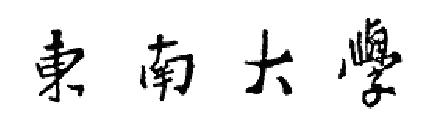
\includegraphics{figures/seu-text-logo} \\
		  \vspace*{60pt}
		  \yihao\hei \bachelortitle \\
		  \vspace*{60pt} \xiaoerhao\song \titlepre \erhao\song
		  \underline{\makebox[18em][s]{\hspace{1em}%
                      \makebox[16em][c]{\fs\@title}}} \\
		  \vspace*{40pt}

		  \renewcommand{\arraystretch}{1.5}
                  \setlength{\tabcolsep}{0pt}
		  \begin{tabular}{clcl}
			  \sanhao\fs
			  \underline{\makebox[8em][s]{\makebox[8em][c]{\@department}}} &
			  \sanhao
			  \departmentpre &
			  \sanhao\fs
			  \underline{\makebox[\@majorlen][s]{\makebox[\@majorlen][c]{\@major}}} &
			  \sanhao
			  \majorpre \\
                        \end{tabular}
                        
                        \vspace*{100pt}

                        \renewcommand{\baselinestretch}{1.38}
                        \renewcommand{\arraystretch}{1.5}
                        \setlength{\tabcolsep}{0pt}
                        \begin{tabular}{c}
			  \sanhao\studentidpre\quad\underline{%
                            \makebox[20em][s]{\makebox[20em][c]{\textsf{\@studentid}}}} \\
			  \sanhao\studentnamepre\quad\underline{\makebox[20em][s]{
                              \makebox[20em][c]{\fs{\@author}}}} \\
			  \sanhao\advisorpre\quad\underline{\makebox[20em][s]{%
                              \hspace{6em}\makebox[4em][c]{\fs{\@advisorname}}%
                              \makebox[4em][r]{\fs{\@advisortitle}}}}
                          \\
                          \ifbcoadvisor
                          \sanhao\coadvisorpre\quad\underline{\makebox[20em][s]{%
                              \hspace{6em}\makebox[4em][c]{\fs{\@coadvisorname}}%
                              \makebox[4em][r]{\fs{\@coadvisortitle}}}} \\
                          \fi
			  \sanhao\durationpre\quad\underline{\makebox[20em][s]{
                              \makebox[20em]{\textsf{\@duration}}}} \\
			  \sanhao\addresspre\quad\underline{\makebox[20em][s]{
                              \makebox[20em][c]{\fs{\@address}}}} \\
                        \end{tabular}

		  \vfill

		  \sanhao\today
	  \end{center}
  \end{titlepage}
  }
\fi
%    \end{macrocode}
% \end{macro}
% 
% \subsubsection{英文封面}
% \begin{macro}{\englishcover}
%    \begin{macrocode}
\newcommand{\englishcover}{
  \thispagestyle{empty}%
  \begin{spacing}{1.0}\begin{center}
      ~\\%
      \begin{spacing}{1.5}\LARGE\textrm{\@titleeng}\end{spacing}%
      \normalsize{\@subtitleeng}

      \vspace{1.0in}%
      {\large
        {A Dissertation Submitted to}\\
        {\universitynameeng}\\
        {For the Academic Degree of \academicdegreeeng}\\
        {\vspace{0.5in}}%
        {BY}\\
        {\@authoreng}\\
        {\vspace{0.5in}}%
        {Supervised by:}\\
        {\@advisortitleeng\  \@advisornameeng}\\
        \ifbcoadvisor
        {and}\\
        {\@coadvisortitleeng\  \@coadvisornameeng}\\
        \else
        \fi
        {\vspace{0.5in}}%
        {\vfill}
        {\@departmenteng}\\
        {\universitynameeng}\\
        {\@submitdateeng}\\
      }%
    \end{center}\end{spacing}%
  \clearpage%
}
%    \end{macrocode}
% \end{macro}
% 
% \subsection{摘要和关键词}
% \begin{environment}{abstract}\IndexEnv{abstract}
%    \begin{macrocode}
\newenvironment{abstract}[1]
{
  \newcommand{\@keywords}{#1}
  \cleardoublepage
  \phantomsection
  \addcontentsline{toc}{chapter}{\@abstracttitletoc}
  \chapter*{\@abstracttitle}
}{
  \begin{description}
  \item[关键词:] \@keywords
  \end{description}
}
%    \end{macrocode}
% \end{environment}
% 
% \begin{environment}{englishabstract}\IndexEnv{englishabstract}
%    \begin{macrocode}
\newenvironment{englishabstract}[1]
{
  \newcommand{\@keywords}{#1}
  \hypersetup{pdfkeywords={\@keywords}}
  \cleardoublepage
  \phantomsection
  \addcontentsline{toc}{chapter}{Abstract}
  \chapter*{Abstract}
}{
  \begin{description}
  \item[Keywords:] \@keywords
  \end{description}
}
%    \end{macrocode}
% \end{environment}
% 
% \subsection{本论文专用术语的注释表}
% 本论文专用术语(符号、变量、缩略词等)的注释表(任选)
% \begin{environment}{terminology}\IndexEnv{terminology}
%    \begin{macrocode}
\newenvironment{terminology}[1][\@terminologytitle]
{
  \cleardoublepage
  \phantomsection
  \addcontentsline{toc}{chapter}{#1}
  \chapter*{#1}
  \song\wuhao
}{
}
%    \end{macrocode}
% \end{environment}
% 
% \section{正文}
% \begin{environment}{Main}\IndexEnv{Main}
%    \begin{macrocode}
\newenvironment{Main}
{
  {\song\sihao\tableofcontents} %目录部分字体可采用4号宋体。

  \pagestyle{seustyle}
  \mainmatter % 开始正文部分
  \song
  \ifbachelordegree
  \xiaosihao
  \else
  \wuhao
  \fi
}{
  \backmatter % 开始正文之后的部分
}
%    \end{macrocode}
% \end{environment}
%
% \subsection{图、表浮动设置} 
% 放宽松浮动的比例参数
\renewcommand{\textfraction}{0.15}
\renewcommand{\topfraction}{0.85}
\renewcommand{\bottomfraction}{0.65}
\renewcommand{\floatpagefraction}{0.8}
%
% \section{参考文献}
% 引用参考文献,上标形式
% \begin{macro}{\cite}\IndexCmd{cite}
%    \begin{macrocode}
\let\originalcite=\cite
\renewcommand{\cite}[1]{\textsuperscript{\originalcite{#1}}}
%    \end{macrocode}
% \end{macro}
% 普通形式
% \begin{macro}{\citet}\IndexCmd{citet}
%    \begin{macrocode}
\renewcommand{\citet}[1]{\originalcite{#1}}
%    \end{macrocode}
% \end{macro}
% 
% 定义参考文献样式
%    \begin{macrocode}
\bibliographystyle{seuthesis}
\makeatletter                   % Reference list option change
\renewcommand\@biblabel[1]{#1}  %   from [1] to 1
\makeatother                    %
%</cls> 
%    \end{macrocode}

% \section{正文之后部分}

% \section{中文关键字映射}
% 将包含中文的代码放在\texttt{seuthesis-*.cfg}中,可以直接转换成不同版
% 本的编码,可以只要一份代码实现两种编码格式。
% \subsection{正文之前部分}
%    \begin{macrocode}
%<*cfg>      
\ProvidesFile{seuthesis.cfg}
\makeatletter
\newcommand{\universityname}{东南大学}
\newcommand{\universitynameeng}{Southeast University}
\newcommand{\secretlevelpre}{密级}
\newcommand{\categorynumberpre}{分类号}
\newcommand{\studentidpre}{学号}
\newcommand{\authorpre}{研究生姓名:}
\newcommand{\advisorpre}{导~~师~~姓~~名:}
\newcommand{\appdegreepre}{申请学位级别}
\newcommand{\majorpre}{学科专业名称}
\newcommand{\submitdatepre}{论文提交日期}
\newcommand{\defenddatepre}{论文答辩日期}
\newcommand{\authorizeorganizationpre}{学位授予单位}
\newcommand{\@authorizeorganization}{~~东~南~大~学~~}
\newcommand{\authorizedatepre}{学位授予日期}
\newcommand{\committeechairpre}{答辩委员会主席}
\newcommand{\readerpre}{评~~~~~~~~~阅~~~~~~~~~人}
\newcommand{\@abstracttitle}{摘\quad 要}
\newcommand{\@abstracttitletoc}{摘要}
\newcommand{\@terminologytitle}{本论文专用术语的注释表}
\renewcommand{\bibname}{参考文献}
% 本科论文需要
\newcommand{\addresspre}{设计地点}
\newcommand{\bachelortitle}{毕业设计(论文)报告}
\newcommand{\durationpre}{起讫日期}
\newcommand{\coadvisorpre}{顾问老师}

\ifbachelordegree
\newcommand{\@appdegree}{学士}
\newcommand{\academicdegreeeng}{Bachelor of Engineering}
\newcommand{\titlepre}{题目\quad}
\newcommand{\departmentpre}{院(系)}
\renewcommand{\majorpre}{专\quad 业}
\renewcommand{\studentidpre}{学\hspace*{2.3em}号}
\newcommand{\studentnamepre}{学生姓名}
\renewcommand{\advisorpre}{指导教师}
\else\ifmasterdegree
\newcommand{\@appdegree}{硕士}
\newcommand{\academicdegreeeng}{Master of Engineering}\relax
\else
\newcommand{\@appdegree}{博士}
\newcommand{\academicdegreeeng}{Doctor of Engineering}\relax
\fi
\fi
\newcommand{\academicdegree}{\@appdegree学位论文}
\makeatother
%    \end{macrocode}
% 
% \subsubsection{论文独创性声明和使用授权声明内容}
% 
% \begin{macro}{\signline}
%   签名的横线
%    \begin{macrocode}
\newcommand{\signline}{\underline{\makebox[2.5cm][s]{}}}
%    \end{macrocode}
% \end{macro}
% 
% \begin{macro}{\seudeclare}
%    \begin{macrocode}
\newcommand{\seudeclare}{
  \begin{center}
    \hei\sanhao{东南大学学位论文独创性声明}
  \end{center}
  
  \xiaosihao\parindent2em{本人声明所呈交的学位论文是我个人在导师指导下
    进行的研究工作及取得的研究成果。尽我所知,除了文中特别加以标注和致
    谢的地方外,论文中不包含其他人已经发表或撰写过的研究成果,也不包含
    为获得东南大学或其它教育机构的学位或证书而使用过的材料。与我一同工
    作的同志对本研究所做的任何贡献均已在论文中作了明确的说明并表示了谢
    意。}
  \\
  \begin{flushright}
    研究生签名:\signline 日~期:\signline
  \end{flushright}

  {\vspace{1in}}

  \begin{center}
    \hei\sanhao{东南大学学位论文使用授权声明}
  \end{center}
  
  \xiaosihao\parindent2em{东南大学、中国科学技术信息研究所、国家图书馆
    有权保留本人所送交学位论文的复印件和电子文档,可以采用影印、缩印或
    其他复制手段保存论文。本人电子文档的内容和纸质论文的内容相一致。除
    在保密期内的保密论文外,允许论文被查阅和借阅,可以公布(包括刊
    登)论文的全部或部分内容。论文的公布(包括刊登)授权东南大学研究生
    院办理。}
  \\
  \begin{flushright}
    研究生签名:\signline 导师签名:\signline 日~期:\signline
  \end{flushright}
}
%    \end{macrocode}
% \end{macro}
% 
% \subsubsection{目录}
%    \begin{macrocode}
\renewcommand{\contentsname}{目\quad 录}
\titlecontents{chapter}[0pt]{\vspace{.5\baselineskip}\bfseries}
{第\CJKnumber{\thecontentslabel}章\quad}{}
{\hspace{.5em}\titlerule*[10pt]{$\cdot$}\contentspage}
%    \end{macrocode}
% 
% \subsection{正文}
% \subsection{章节标题}
% 三号黑体居中
%    \begin{macrocode}
\titleformat{\chapter}[hang]{\centering\hei\sanhao}{\chaptername}{1em}{}%三号黑体居中
\renewcommand{\chaptername}{第\CJKnumber{\thechapter}章}
\titleformat{\section}[hang]{\song\sihao\bfseries}{\thesection}{1em}{}%四号宋体(粗体)居左
\titleformat{\subsection}[hang]{\song\xiaosihao}{\thesubsection}{1em}{}% 小四
\setcounter{secnumdepth}{3}
\titleformat{\subsubsection}[hang]{\song\xiaosihao}{\thesubsubsection}{1em}{}% 小四
%    \end{macrocode}
% \begin{macro}{\refsec}\IndexCmd{refsec}
%    \begin{macrocode}
\newcommand{\refsec}[1]{\hyperref[#1]{\ref*{#1}节}}
%    \end{macrocode}
% \end{macro}
% 
% \begin{macro}{\refchapter}\IndexCmd{refchapter}
%    \begin{macrocode}
\newcommand{\refchapter}[1]{\hyperref[#1]{第\ref*{#1}章}}
%    \end{macrocode}
% \end{macro}
% 
% \subsubsection{图、表}
% \begin{quote}
%   表格名及图名用5号宋体
% \end{quote}
%    \begin{macrocode}
\renewcommand{\captionlabeldelim}{} % 去掉图标签后的冒号
\renewcommand{\captionfont}{\song\wuhao} % 表格名及图名用5号宋体
\renewcommand{\figureautorefname}{图}
\renewcommand{\prefigurename}{\song\wuhao图}
\renewcommand{\postfigurename}{}
\renewcommand{\listfigurename}{插图目录}
\renewcommand{\tableautorefname}{表}
\renewcommand{\pretablename}{\song\wuhao表}
\renewcommand{\posttablename}{}
\renewcommand{\listtablename}{表格目录}
\renewcommand{\equationautorefname}{式}
\makeatletter
\renewcommand\fps@figure{htbp} % 设置图浮动的默认参数
\renewcommand\fps@table{htbp}
\makeatother
%    \end{macrocode}
% 
% \subsection{正文之后部分}
% 
%    \begin{macrocode}
\IndexPrologue{\chapter*{索\quad 引}}
% 
%</cfg> 
%    \end{macrocode}
% 
% \Finale \RecordChanges

% \endinput
% Local Variables: 
% mode: doctex
% TeX-master: t
% End: 
